%FOR PDFLATEX USE ONLY
\documentclass[a4paper,12pt]{article}

\usepackage{amssymb,amsmath}

\usepackage[margin=2cm]{geometry}
\usepackage[unicode]{hyperref}
\usepackage[pdftex]{graphicx}
\usepackage{cmlgc}

\usepackage{array}

\usepackage{wrapfig}
\usepackage{array}
\usepackage{lipsum}
\usepackage{esvect}
\usepackage{hyperref}

\usepackage{subfig}
\usepackage{calc}
\usepackage{pgfplots,tikz,circuitikz}
\usepackage{pgfplotstable}
\usepackage{tkz-euclide}

\usepackage{centernot}
\usepackage{cancel}

\usepackage{mathtext}
\usepackage[T1,T2a]{fontenc}
\usepackage[utf8]{inputenc}
\usepackage[english, bulgarian, russian]{babel}
\usepackage{tikz}
\usepackage{pgfplots}
\usepackage[export]{adjustbox}
\usepackage[left=2cm,right=2cm,
    top=2cm,bottom=2cm,bindingoffset=0cm]{geometry}
\usepackage{indentfirst}
\usepackage{braket}

\begin{document}

\begin{center}
  \LARGE{Работа 2.5.1}\\[0.2cm]
  \LARGE{Измерение коэффициента поверхностного натяжения жидкости.}\\[0.2cm]
  \large{Панферов Андрей}\\[0.2cm]
\end{center}

\textbf{Цель работы:} 1) измерение температурной зависимости  коэффициента поверхностного натяжения дистиллированной воды с использованием известного коэффициента поверхностного натяжения спирта;  2) определение полной поверхностной энергии  и теплоты, необходимой для изотермического образования единицы  поверхности жидкости  при различной температуре. 

\textbf{В работе используются:} прибор  Ребиндера  с термостатом и микроманометром; исследуемые жидкости; стаканы.

\begin{center}
	\lagre{\textbf{Теоретические сведения}}
\end{center}

Наличие поверхностного слоя приводит к различию давлений по разные стороны от искривленной границы раздела двух сред.  Для сферического пузырька с воздухом  внутри жидкости избыточное давление даётся формулой Лапласа:

\begin{equation}
\Delta P = P_{inside} - P_{outside} = \frac{2\sigma}{r},
\end{equation}

где $\sigma$ – коэффициент поверхностного натяжения, $P_{inside}$ и $P_{outside}$ – давление внутри пузырька и снаружи, r – радиус кривизны поверхности раздела двух фаз. Эта формула лежит в основе предлагаемого метода определения коэффициента поверхностного натяжения жидкости. Измеряется давление $\Delta P$, необходимое для выталкивания в жидкость пузырька воздуха.

\begin{center}
	\lagre{\textbf{Экспериментальная установка}}
\end{center}

Исследуемая жидкость (дистиллированная вода) наливается в сосуд (колбу) В. Тестовая жидкость  (этиловый спирт) наливается  в сосуд Е.  При измерениях  колбы герметично закрываются  пробками.   Через одну из двух пробок  проходит полая металлическая игла С. Этой пробкой закрывается сосуд, в котором  проводятся измерения. Верхний конец иглы открыт в атмосферу, а нижний погружен в жидкость. Другой сосуд герметично закрывается второй пробкой. При создании достаточного  разряжения воздуха в колбе с иглой пузырьки воздуха начинают пробулькивать через жидкость. Поверхностное натяжение можно определить по величине разряжения ∆P (1), необходимого для прохождения пузырьков (при известном радиусе иглы).

\bigskip

Разряжение в системе создается с помощью аспиратора А. Кран К2 разделяет две полости аспиратора. Верхняя полость при закрытом кране К2  заполняется водой. Затем кран К2 открывают и заполняют водой  нижнюю полость  аспиратора.  Разряжение воздуха создается в нижней полости  при открывании крана К1, когда  вода вытекает из неё по каплям. В колбах В и С, соединённых трубками с нижней полостью аспиратора,  создается такое же пониженное давление. Разность давлений в полостях с разряженным воздухом и атмосферой измеряется спиртовым микроманометром (устройство микроманометра описано в Приложении). 
Для стабилизации температуры исследуемой жидкости через рубашку D колбы В непрерывно прогоняется вода из термостата.

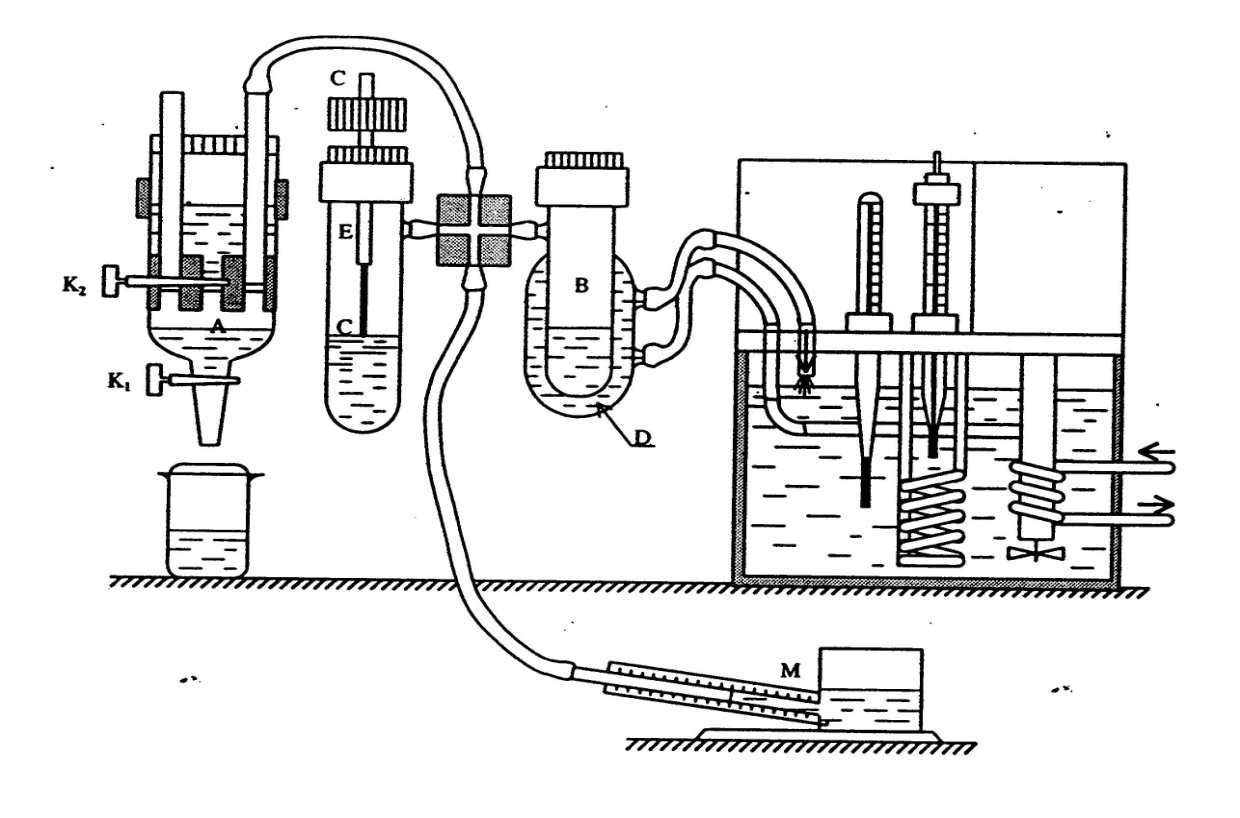
\includegraphics[width=1\textwidth]{Scheme.jpg}

Обычно кончик иглы лишь касается поверхности жидкости, чтобы исключить влияние гидростатического давления столба жидкости. Однако при измерении температурной зависимости коэффициента поверхностного натяжения возникает ряд сложностей. Во-первых, большая теплопроводность металлической трубки приводит к тому, что температура на конце трубки заметно ниже, чем в глубине жидкости. Во-вторых, тепловое расширение поднимает уровень жидкости при увеличении температуры. 
Обе погрешности можно устранить, погрузив кончик трубки до самого дна. Полное давление, измеренное при этом микроманометром, $P = \Delta P + \rho gh$. Заметим, что $\rho gh$ от температуры практически не зависит, так как подъём уровня жидкости компенсируется уменьшением её плотности (произведение ρh определяется массой всей жидкости и поэтому постоянно). Величину  $\rho gh$ следует измерить двумя способами. Во-первых, замерить величину $P1 = \Delta P'$, когда кончик трубки только касается поверхности жидкости. Затем при этой же температуре опустить иглу до дна и замерить $P2 = \rho gh + \Delta P"$ ($\Delta P' ,\: \Delta P"$ – давление Лапласа). Из-за  несжимаемости  жидкости можно положить $\Delta P' = \Delta P"$ и тогда $\rho gh = P2 -P1$. Во-вторых, при измерениях $Р1$ и $Р2$ замерить линейкой  глубину погружения иглы $h$. Это можно сделать, замеряя расстояние между верхним концом иглы и любой неподвижной частью прибора при положении иглы на поверхности и в глубине колбы.

\begin{center}
	\lagre{\textbf{Измерения}}
\end{center}

Проведем измерения для спирта. Для этого установим частоту падения капель из аспиратора около 1 капли в 5 секунд. Измерим максимальное добавочно давление в системе и занесем данные в \textit{Tаблицу 1}(пересчет единиц шкалы в паскали произведем потом).

\bigskip

Далее вынем иглу, просушим ее и измерим микроскопом ее диаметр (внутренний):

\begin{equation*}
d = 0.95 \pm 0.05 mm
\end{equation*}

Из табличного значения коэффициента поверхностного натяжения спирта $\sigma = 22.8 \: \: мн/м$ по \textit{Формуле (1)} плучим:

\begin{equation*}
d = 0.93\pm 0.02 mm
\end{equation*}

\bigskip

Затем установим иглу в воду так, чтобы она едва касалась воды. Проведя измерения давления и занеся результаты в \textit{Tаблицу 1}, опустим иглу до дна, предварительно измерив высоту. Вновь измерим высоту

\begin{align*}
 h1&=17.5 \pm 0.5 mm & h2&=10.5 \pm 0.5 mm\\
\end{align*} 

\bigskip

Проведем серию измерений $P2$ для различных температур воды, регулируемых термостатом, занесем результаты в \textit{Tаблицу 1}.

\bigskip

\begin{center}
	\lagre{\textbf{Обработка данных}}
\end{center}

\smallskip

Проведем пересчет экспериментальных данных для нахождения $\sigma(T)$, оценим погрешности.

\smallskip

Построим график зависимости $\sigma(T)$

\smallskip

Из график \textit{методом наименьших квадратов} найдем:

\smallskip

\begin{equation*}
	\frac{d\sigma}{dT} = (-0.12 \pm 0.01) мН \cdot м / С
\end{equation*}

Сравним с табличным:

\begin{equation*}
	\frac{d\sigma_т}{dT} = -0.17 мН \cdot м / С
\end{equation*}

\bigskip

\begin{center}
	\lagre{\textbf{Вывод}}
\end{center}

Теория точно описывает вид наблюдаемых зависимостей, хоть численно и отличается на величину, значительно превышающую оцененную погрешность измерений, что указывает на низкую точность представленного метода измерений, которая может быть связана с неоюходимостью учета сложных не квазистационарных процессах, происходящих при пробулькивании пузырька через жидкость.


\newpage

\begin{center}
	\lagre{\textbf{Данные}}
\end{center}

\begin{center}
\begin{table}[h!]
\centering
\begin{tabular}{|c||c||c|c|c|c|c|c|c|c|c|c|}
\hline
Спирт                  & \multicolumn{1}{l|}{}         & \multicolumn{10}{c|}{Вода}                                                                                                                                                                                                                    \\ \hline
21.3                   & T, C                          & 21,3                  & 21,3                  & 25,2                  & 30,2                  & 35,2                  & 40,2                  & 45,2                  & 50,2                  & 55,2                  & 60,2                  \\ \hline
\hline
P1                &                               & P1                    & P2                    & P2                    & P2                    & P2                    & P2                    & P2                    & P2                    & P2                    & P2                    \\ \hline
49                     &                               & 138                   & 172                   & 173                   & 172                   & 171                   & 169                   & 167                   & 166                   & 165                   & 163                   \\ \hline
49                     &                               & 138                   & 172                   & 173                   & 172                   & 171                   & 169                   & 166                   & 166                   & 165                   & 164                   \\ \hline
49                     &                               & 138                   & 172                   & 173                   & 172                   & 170                   & 169                   & 167                   & 166                   & 165                   & 164                   \\ \hline
49                     &                               & 138                   & 172                   & 173                   & 172                   & 170                   & 169                   & 167                   & 166                   & 165                   & 163                   \\ \hline
49                     &                               & 138                   & 172                   & 173                   & 172                   & 171                   & 169                   & 167                   & 166                   & 165                   & 163                   \\ \hline
\hline
94 & $P1_{ср}$, Па & 266 & 330 & 332 & 330 & 328 & 324 & 320 & 319 & 318 & 314 \\ \hline
2  & $\Delta P1_{ср}$, Па & 2   & 2   & 2   & 2   & 3   & 2   & 3   & 2   & 2   & 3   \\ \hline
21.8   & $\sigma$, $мПа \cdot м$         &  61.8   &   61.8  &   62.3  &  61.8   &   61.4    &  60.4   &   59.5    &   59.3  &   59.0  &   58.1    \\
\hline
0.5    & $\Delta\sigma$, $мПа \cdot м$ & 0.5 & 0.5 & 0.5 & 0.5 & 0.5 & 0.5 & 0.5 & 0.5 & 0.5 & 0.5 \\          
\hline
22.3   & $\sigma_т$, $мПа \cdot м$       &  72.1   &  72.1   &   71.7  &   71.2  &   70.4   &   69.6    &  68.8   &   67.9    &   67.0  &   66.2    \\   
\hline
\end{tabular}
\caption{Измерения}
\label{tab:my-table}
\end{table}
\end{center}

\begin{minipage}{.5\textwidth}
\begin{tikzpicture}[scale=1]
	\begin{axis}[
		axis lines = left,
    	xlabel = {T, C},
    	ylabel = {$\sigma$, $мПа\cdotм$},
    	ylabel style={red, scale=0.7},
    	xlabel style={red, scale=0.7},
    	%xmin=0, xmax=9,
    	title={Зависимость $\sigma$ от $T$},
    	legend style={at={(0.03,-0.4)},anchor=west}
		]
		\addplot+[blue, only marks]  plot[
			error bars/.cd,
			y dir=both,
			y fixed = 0.6,
			x dir = both,
			x fixed = 0.1,
		]
		coordinates
		{(21.3, 61.8) (25.2, 62.3) (30.2, 61.8) (35.2, 61.4) (40.2, 60.4) (45.2, 59.5) (50.2, 59.3) (55.2, 59) (60.2, 58.1)};
		\addlegendentry{Экспериментальные точки};
		\addplot[color=red, domain=20:60]{80.2693333-14.88 + -0.1204762 * x};
		\addlegendentry{$\sigma$};
		%\addplot[color=green, domain=20:60]{80.2693333-14.88 + -0.1204762 * x - (273 + x) * (-0.1204762)};
		%\addlegendentry{$U_п/П$};
		%\addplot[color=yellow, domain=20:60]{- (273 + x) * (-0.1204762)};
		%\addlegendentry{$q$};
		

	\end{axis}
\end{tikzpicture}
\end{minipage}
\begin{minipage}{.5\textwidth}
\begin{tikzpicture}[scale=1]
	\begin{axis}[
		axis lines = left,
    	xlabel = {T, C},
    	ylabel = {$\sigma$, $мПа\cdotм$},
    	ylabel style={red, scale=0.7},
    	xlabel style={red, scale=0.7},
    	%xmin=0, xmax=9,
    	title={Зависимость $\sigma$ от $T$},
    	legend style={at={(0.03,-0.4)},anchor=west}
		]
		\addplot+[blue, only marks]  plot[
			error bars/.cd,
			y dir=both,
			y fixed = 0.6,
			x dir = both,
			x fixed = 0.1,
		]
		coordinates
		{(21.3, 61.8) (25.2, 62.3) (30.2, 61.8) (35.2, 61.4) (40.2, 60.4) (45.2, 59.5) (50.2, 59.3) (55.2, 59) (60.2, 58.1)};
		\addlegendentry{Экспериментальные точки};
		\addplot[color=red, domain=20:60]{80.2693333-14.88 + -0.1204762 * x};
		\addlegendentry{$\sigma$};
		\addplot[color=green, domain=20:60]{80.2693333-14.88 + -0.1204762 * x - (273 + x) * (-0.1204762)};
		\addlegendentry{$U_п/П$};
		\addplot[color=yellow, domain=20:60]{- (273 + x) * (-0.1204762)};
		\addlegendentry{$q$};
		

	\end{axis}
\end{tikzpicture}
\end{minipage}


\end{document}